% Created 2020-07-01 mié 12:04
% Intended LaTeX compiler: pdflatex
\documentclass[presentation,aspectratio=169]{beamer}
\usepackage[utf8]{inputenc}
\usepackage[T1]{fontenc}
\usepackage{graphicx}
\usepackage{grffile}
\usepackage{longtable}
\usepackage{wrapfig}
\usepackage{rotating}
\usepackage[normalem]{ulem}
\usepackage{amsmath}
\usepackage{textcomp}
\usepackage{amssymb}
\usepackage{capt-of}
\usepackage{hyperref}
\usepackage{khpreamble}
\usepackage{amssymb}
\DeclareMathOperator{\shift}{q}
\DeclareMathOperator{\diff}{p}
\usetheme{default}
\author{Kjartan Halvorsen}
\date{2020-07-02}
\title{Control Computarizado - La transformada z}
\hypersetup{
 pdfauthor={Kjartan Halvorsen},
 pdftitle={Control Computarizado - La transformada z},
 pdfkeywords={},
 pdfsubject={},
 pdfcreator={Emacs 26.3 (Org mode 9.3.6)}, 
 pdflang={English}}
\begin{document}

\maketitle

\section{Intro}
\label{sec:orge149df4}
\section{Discrete-time system example}
\label{sec:org89d92a9}

\section{Zero-order hold, or step-invariant sampling preview}
\label{sec:orgceca1c8}

\begin{frame}[label={sec:org7e39616}]{El mundo según el controlador discreto}
\begin{center}
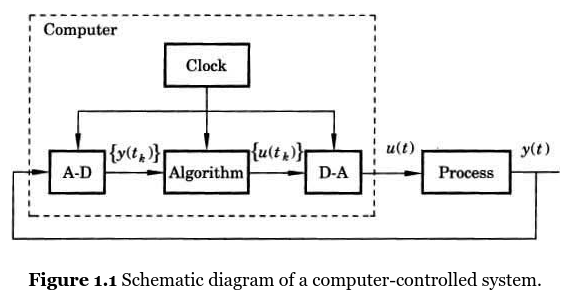
\includegraphics[width=0.6\linewidth]{../../figures/fig1-1-schematic.png}
\end{center}
\end{frame}

\begin{frame}[label={sec:org59e53f9}]{Discretizacion invariante al paso (\emph{step-invariant} o \emph{zero-order-hold sampling})}
El idea es muestrear la respuesta de paso del sistema continuo para obtener un modelo discreto que es \alert{exacto} (en los instantes de muestreo) para señales de entrada que son combinaciones de pasos (funciones constantes por partes)

\begin{center}
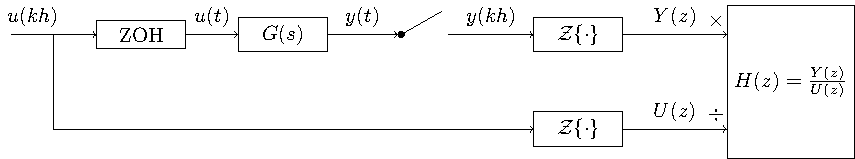
\includegraphics[width=0.9\linewidth]{../../figures/invariant-sampling.pdf}
\end{center}

\[ u(t) = \begin{cases} 1, & t \ge 0\\0, & t<0 \end{cases} \]
\end{frame}

\begin{frame}[label={sec:orgc132753}]{Porqué discretizacion invariante al paso?}
A piecewise constant (stair-case shaped) function can be written as a sum of delayed step-responses!
\begin{LaTeX}
\begin{center}
  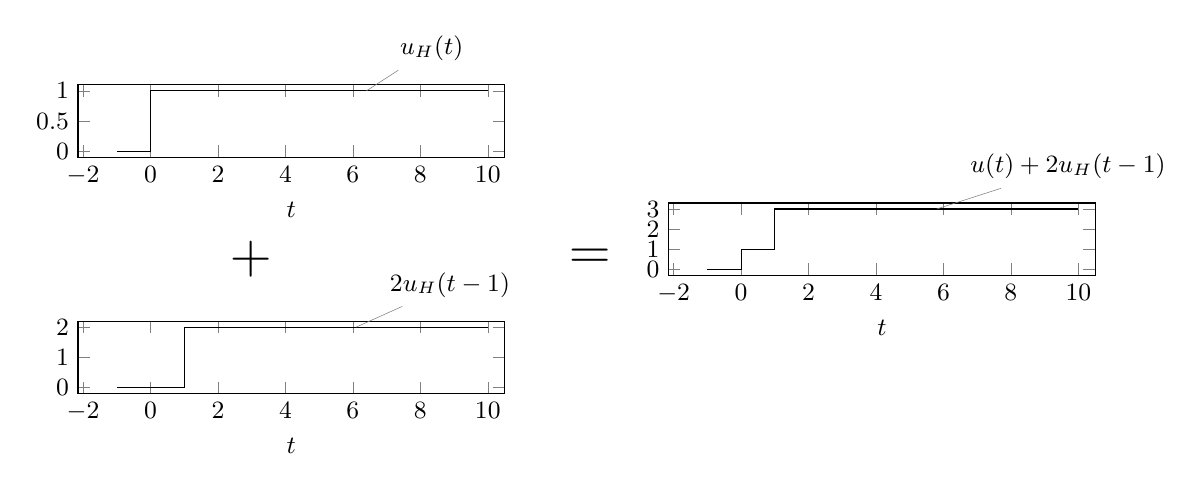
\begin{tikzpicture}
    \small
    \begin{axis}[
      clip = false,
      width=7cm,
      height=2.5cm,
      yshift=1.5cm,
      xlabel={$t$},
      ylabel={},
      xmax=10.5,
      ]
      \addplot+[black, no marks] coordinates {(-1,0) (0,0) (0,1) (10,1) } node[pos=0.7,coordinate, pin=40:$u_H(t)$] {};
    \end{axis}
    \begin{axis}[
      clip=false,
      width=7cm,
      height=2.5cm,
      yshift=-1.5cm,
      xlabel={$t$},
      ylabel={},
      xmax=10.5,
      ]
      \addplot+[black, no marks] coordinates {(-1,0) (1,0) (1,2) (10,2) } node[pos=0.7,coordinate, pin=40:$2u_H(t-1)$] {};;
    \end{axis}
    \begin{axis}[
      clip=false,
      width=7cm,
      height=2.5cm,
      xshift=7.5cm,
      xlabel={$t$},
      ylabel={},
      xmax=10.5,
      ]
      \addplot+[black, no marks] coordinates {(-1,0) (0,0) (0,1) (1,1) (1,3) (10,3) }  node[pos=0.7,coordinate, pin=40:$u(t) + 2u_H(t-1)$] {};;
    \end{axis}

    \node at (2.2,0.2) {\huge  +};
    \node at (6.5,0.2) {\huge  =};

  \end{tikzpicture}
\end{center}
\end{LaTeX}
\end{frame}


\begin{frame}[label={sec:org7fe2f9c}]{Why is step-invariant sampling a good idea? (contd)}
Due to the system being LTI (linear time-invariant), the output to a sum of delayed step functions, is the same sum of delayed step-responses.

\begin{LaTeX}
\begin{center}
  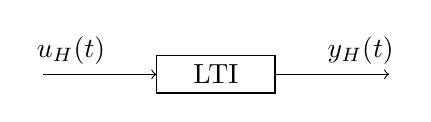
\begin{tikzpicture}[node distance=20mm, block/.style={rectangle, draw, minimum width=15mm, }]

    \node[coordinate] (input) {};
    \node[block, right of=input, node distance=22mm] (lti) {LTI};
    \node[coordinate, right of=lti, node distance=22mm] (output) {};

    \draw[->] (input) -- node[above, near start] {$u_H(t)$} (lti);
    \draw[->] (lti) -- node[above, near end] {$y_H(t)$} (output);
  \end{tikzpicture}
\end{center}
\end{LaTeX}
Hence, \(u(t) = \sum_{i} \alpha_i u_H(t-\tau_i)\) has the response \(y(t)=\). 
\end{frame}

\begin{frame}[label={sec:org0bda2ea}]{Why is step-invariant sampling a good idea? (contd)}
Due to the system being LTI (linear time-invariant), the output to a sum of delayed step functions, is the same sum of delayed step-responses.

\begin{LaTeX}
\begin{center}
  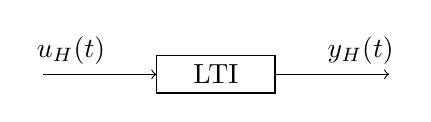
\begin{tikzpicture}[node distance=20mm, block/.style={rectangle, draw, minimum width=15mm, }]

    \node[coordinate] (input) {};
    \node[block, right of=input, node distance=22mm] (lti) {LTI};
    \node[coordinate, right of=lti, node distance=22mm] (output) {};

    \draw[->] (input) -- node[above, near start] {$u_H(t)$} (lti);
    \draw[->] (lti) -- node[above, near end] {$y_H(t)$} (output);
  \end{tikzpicture}
\end{center}
\end{LaTeX}
Hence, \(u(t) = \sum_{i} \alpha_i u_H(t-\tau_i)\) has the response \(y(t) = \sum_i \alpha_i y_H(t-\tau_i)\). 

\alert{If the sampling method is exact for step input signals, it will also be exact for piecwise-constant step input signals, and this is exactly what the ZOH-block produces!}
\end{frame}

\section{Zero-order hold sampling procedure}
\label{sec:org14970b5}
\begin{frame}[label={sec:org22b73b4}]{Impulse- step- and ramp-invariant sampling}
\begin{center}
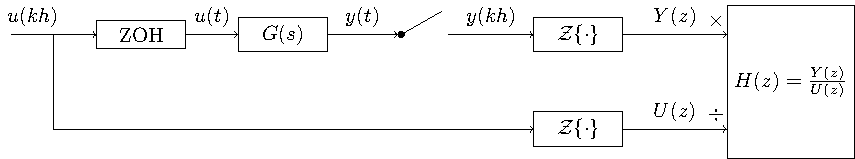
\includegraphics[width=0.9\linewidth]{../../figures/invariant-sampling.pdf}
\end{center}

\begin{itemize}
\item Impulse-invariant sampling: \(u(t) = \delta(t)\)
\item Step-invariant sampling (zero order hold): \(u(t) = \begin{cases} 1, & t \ge 0\\0, & t<0 \end{cases}\)
\item Ramp-invariant sampling: \(u(t) = \begin{cases} t, & t \ge 0\\0, & t<0 \end{cases}\)
\end{itemize}
\end{frame}

\begin{frame}[label={sec:orgeeea6e6}]{Step-invariant sampling, or zero-order-hold sampling}
Let the input to the continuous-time system be a step \(u(t)=\stepfcn,\) which has Laplace transform \(U(s)=\frac{1}{s}.\) In the Laplace-domain we get
\[Y(s) = G(s)\frac{1}{s}\]
\begin{enumerate}
\item Obtain the time-response by inverse Laplace: \(y(t)=\laplaceinv{Y(s)}\)
\item Sample the time-response to obtain the sequence \(y(kh)\) and apply  the z-transform to obtain \(Y(z) = \ztrf{y(kh)}\)
\item Calculate the pulse-transfer function by dividing with the z-transform of the input signal \(U(z) = \frac{z}{z-1}.\) \[H(z) = \frac{Y(z)}{U(z)} = \frac{z-1}{z}Y(z) \]
\end{enumerate}
\end{frame}

\section{Zero-order hold sampling example}
\label{sec:orgb8e6c6a}
\begin{frame}[label={sec:org3040f70}]{Example: First-order system}
Let's apply step-invariant sampling to the system
\[ G(s) = \frac{1}{s + a}. \]
\end{frame}

\begin{frame}[label={sec:orgf92c785}]{Do on your own: The double integrator}
\[ G(s) = \frac{1}{s^2} \]
\end{frame}

\section{The solution to discrete-time systems}
\label{sec:orgc55076c}
\begin{frame}[label={sec:orgc9228fc}]{Another important property of the z-transform}
\end{frame}


\begin{frame}[label={sec:org982df2f}]{The z-transform and the solution to difference equations}
Taking the z-transform of a difference equation 
\[ \left( \shift^2 + a_1\shift + a_2) y_k = \left(b_0\shift^2 + b_1\shift + b_2 \right) u_k\]
gives
\begin{equation*}
\begin{split}
z^{2}Y -z^2y(0) &- zy(1) + a_1zY - a_1zy(0) + a_2Y =\\
&     b_0z^2U -b_0z^2u(0) - b_0zu(1) + b_1zU - b_1zu(0) + b_2U
\end{split}
\end{equation*}

\begin{equation*}
\begin{split}
 Y(z) &= \underbrace{ \frac{ \big( y(0)-b_0u(0)\big) z^2 + \big(y(1)+a_1y(0) - b_0u(1) -b_1u(0)\big) z}{z^2 + a_1z + a_2}}_{\text{transient response}}\\
 & \qquad + \underbrace{\underbrace{\frac{b_0z^2 + b_1z + b_2}{z^2 + a_1z + a_2}}_{\text{pulse-transfer function}}U(z)}_{\text{response to input}}
\end{split}
\end{equation*}
\end{frame}

\begin{frame}[label={sec:org308f283}]{The z-transform and the solution to difference equations}
In general, the output of the discrete-time LTI 

\[ \left( \shift^n + a_1 \shift^{n-1} + \cdots + a_n \right) y(k) = \left( b_0 \shift^m + b_1\shift^{m-1} + \cdots + b_m \right)  u(k) \]

is
\[ Y(z) = \frac{\beta(z)}{A(z)} + \frac{B(z)}{A(z)} U(z) \]

For systems that are intially at rest

\[ Y(z) = \frac{B(z)}{A(z)} U(z)  = G(z) U(z) \]
\end{frame}

\begin{frame}[label={sec:org829f215}]{Convolution in the time-domain is multiplication in the z-domain}
\[ \ztrf{g \ast u)} = \ztrf{g(kh)} \ztrf{u(kh)} = \left(\sum_{k=0}^{\infty} g(kh)z^{-k}\right) \left(\sum_{k=0}^{\infty} u(kh)z^{-k}\right)\]


\begin{LaTeX}
\begin{center}
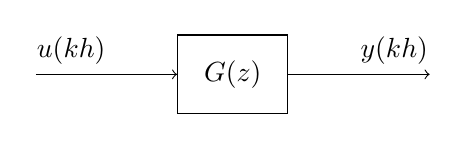
\begin{tikzpicture}[node distance=25mm]
\node[rectangle, draw, minimum height=10mm, minimum width=14mm] (sys) {$G(z)$};
\node[coordinate, left of=sys] (input) {};
\node[coordinate, right of=sys] (output) {};
\draw[->] (input) -- node [near start, above] {$u(kh)$} (sys);
\draw[->] (sys) -- node [near end, above] {$y(kh)$} (output);
\end{tikzpicture}
\end{center}
\end{LaTeX}
\[ y(kh) = g(kh) \ast u(kh) \]
\[ \ztrf{y(kh)} = \ztrf{g(kh) \ast u(kh)} \]
\[ Y(z) = G(z) U(z). \]

The z-transform plays the same role for discrete-time control  systems as the Laplace transform for continuous-time ontrol systems!
\end{frame}
\end{document}